%%%%%%%%%%%%%%%%%%%%%%%%%%%%%%%%%%%%%%%%%%%%%%%%%%%%%%%%%%%%%%%%%%%%%%%%%%%%%%%%%%%%%%%%%%%%%
\chapter{Cellular fibration theorem}\label{chap:cellular_fibration_theorem}
In this chapter, we state the cellular fibration theorem \ref{thm:cellular_fibration}, and apply it to get the module structure of $K$-groups, as shown in Table \ref{table:module_initial}, \ref{table:module_relative} and \ref{table:module_absolute}.
\section{Statement}
We first state one general theorem, and then apply it repeatly to get the cellular fibration theorem.
\begin{theorem}[{Glueing theorem, \cite[Lemma 5.5.1(a)]{chriss1997representation}}]\label{thm:glueing_theorem}\index{glueing theorem}
Suppose the triple $(X,Y,\pi)$ satisfies assumption \eqref{eq:assumption2}. For a $G$-equivariant closed embedding $i:Z \hookrightarrow Y$, define $U:=Y \smallsetminus Z$, and $j:U \hookrightarrow Y$ as the open immersion, as follows.
% https://q.uiver.app/?q=WzAsNCxbMCwwLCJaIl0sWzEsMCwiWSJdLFsyLDAsIlUiXSxbMSwxLCJYIl0sWzAsMSwiaSIsMCx7InN0eWxlIjp7InRhaWwiOnsibmFtZSI6Imhvb2siLCJzaWRlIjoidG9wIn19fV0sWzIsMSwiaiIsMix7InN0eWxlIjp7InRhaWwiOnsibmFtZSI6Imhvb2siLCJzaWRlIjoiYm90dG9tIn19fV0sWzEsMywiXFxwaSJdXQ==
\[\begin{tikzcd}
	Z & Y & U \\
	& X
	\arrow["i", hook, from=1-1, to=1-2]
	\arrow["j"', hook', from=1-3, to=1-2]
	\arrow["\pi", from=1-2, to=2-2]
\end{tikzcd}\]

Suppose that $\pi|_U=\pi \circ j: U \longrightarrow X$ realizes $U$ as a $G$-equivariant affine bundle on $X$, so 
$$\pi\big|_U^*: K^G(X) \stackrel{\cong}{\longrightarrow} K^G(U)$$
as $\Rpt(G)$-modules.

\begingroup
\upshape
\begin{enumerate}[(1)]
\item We have a canonical short exact sequence 
% https://q.uiver.app/?q=WzAsNSxbMSwwLCJLXkcoWikiXSxbMiwwLCJLXkcoWSkiXSxbMywwLCJLXkcoVSkiXSxbNCwwLCIwIl0sWzAsMCwiMCJdLFswLDEsImlfKiJdLFsxLDIsImpeKiJdLFsyLDNdLFs0LDBdLFsyLDEsInMiLDAseyJjdXJ2ZSI6LTIsImNvbG91ciI6WzEsMTAwLDYwXSwic3R5bGUiOnsiYm9keSI6eyJuYW1lIjoiZGFzaGVkIn19fSxbMSwxMDAsNjAsMV1dXQ==
\begin{equation}\label{eq:glueing_theorem}
\begin{tikzcd}
	0 & {K^G(Z)} & {K^G(Y)} & {K^G(U)} & 0
	\arrow["{i_*}", from=1-2, to=1-3]
	\arrow["{j^*}", from=1-3, to=1-4]
	\arrow[from=1-4, to=1-5]
	\arrow[from=1-1, to=1-2]
	\arrow["s", color={rgb,255:red,255;green,54;blue,51}, curve={height=-12pt}, dashed, from=1-4, to=1-3]
\end{tikzcd}
\end{equation}
\item If $K^G(X)$ is a free $\Rpt(G)$-module with basis $\{y_1,\ldots y_m\}$, then the short exact sequence \eqref{eq:glueing_theorem} (non-naturally) splits, and
$$K^G(Y) \cong K^G(Z) \oplus K^G(U)$$
as $\Rpt(G)$-modules. The splitting $s$ is defined on basis of $K^G(U)$:
$$s:K^G(U) \longrightarrow K^G(Y) \qquad \pi\big|_U^*(y_l) \longmapsto \iota_{\overline{U},*} \pi\big|_{\overline{U}}^*(y_l)$$
where $\iota_{\overline{U}}$, $\pi\big|_{\overline{U}}$ are defined in the following diagram:
% https://q.uiver.app/?q=WzAsNCxbMCwwLCJVIl0sWzEsMCwiXFxvdmVybGluZXtVfSJdLFsyLDAsIlkiXSxbMiwxLCJYIl0sWzIsMywiXFxwaSJdLFsxLDMsIlxccGlcXGJpZ3xfe1xcb3ZlcmxpbmV7VX19IiwyXSxbMCwzLCJcXHBpXFxiaWd8X3tVfSIsMl0sWzAsMSwiIiwxLHsic3R5bGUiOnsidGFpbCI6eyJuYW1lIjoiaG9vayIsInNpZGUiOiJ0b3AifX19XSxbMSwyLCJcXGlvdGFfe1xcb3ZlcmxpbmV7VX19IiwwLHsic3R5bGUiOnsidGFpbCI6eyJuYW1lIjoiaG9vayIsInNpZGUiOiJ0b3AifX19XV0=
\[\begin{tikzcd}
	U & {\overline{U}} & Y \\
	&& X
	\arrow["\pi", from=1-3, to=2-3]
	\arrow["{\pi\big|_{\overline{U}}}"{pos=0.8,xshift=-3mm}, from=1-2, to=2-3]
	\arrow["{\pi\big|_{U}}"'{pos=0.2,xshift=3mm}, from=1-1, to=2-3]
	\arrow[hook, from=1-1, to=1-2]
	\arrow["{\iota_{\overline{U}}}", hook, from=1-2, to=1-3]
\end{tikzcd}\]

\end{enumerate}
\endgroup
\end{theorem}

In practice, we will use Theorem \ref{thm:glueing_theorem} by repetition.

\begin{defn}[Cellular fibration]
Let $\pi:E \longrightarrow X$ be a $G$-equivariant morphism satisfying the assumption \eqref{eq:assumption2}. A ($G$-equivariant) \textbf{cellular fibration structure}\index{cellular fibration structure} of $E$ is a fibration of closed $G$-equivariant subvarieties
$$\varnothing =E_0 \subseteq E_1 \subseteq \cdots \subseteq E_k=E$$
such that $\pi_j:=\pi\big|_{E_j \smallsetminus E_{j-1}}: E_j \smallsetminus E_{j-1} \longrightarrow X$ is a $G$-equivariant affine bundle over $X$, for any $j \in \{1,\ldots,k \}$.

When $X=\pt$, this filtration is called a \textbf{cellular decomposition}\index{cellular decomposition} of $E$.
\end{defn}

\begin{theorem}[{Cellular fibration theorem, \cite[Lemma 5.5.1]{chriss1997representation}}]\label{thm:cellular_fibration}\index{cellular fibration theorem}
Suppose a $G$-equivariant morphism $\pi: E \longrightarrow X$ has a cellular fibration structure
$$\varnothing =E_0 \subseteq E_1 \subseteq \cdots \subseteq E_k=E$$
and $K^G(X)$ is a free $\Rpt(G)$-module with basis $\{y_1,\ldots,y_m \}$. 

For $j \in \{1,\ldots,k \}$, let $U_j:=E_j \setminus E_{j-1}$, $\overline{U}_j$ denotes the closure of $U_j$ in $E_j$, $\iota_{\overline{U}_j}$ be the embedding of  $\overline{U}_j$ in $E$,  $\pi_{\overline{U}_j}:= \pi\big|_{\overline{U}_j}=\pi \circ \iota$, as follows.
% https://q.uiver.app/?q=WzAsMyxbMCwwLCJcXG92ZXJsaW5le1V9X2oiXSxbMSwwLCJFIl0sWzAsMSwiWCJdLFsxLDIsIlxccGkiLDAseyJzdHlsZSI6eyJib2R5Ijp7Im5hbWUiOiJkYXNoZWQifX19XSxbMCwyLCJcXHBpXFxiaWd8X3tcXG92ZXJsaW5le1V9X2p9IiwyXSxbMCwxLCJcXGlvdGFfe1xcb3ZlcmxpbmV7VX1fan0iLDAseyJzdHlsZSI6eyJ0YWlsIjp7Im5hbWUiOiJob29rIiwic2lkZSI6InRvcCJ9fX1dXQ==
\[\begin{tikzcd}
	{\overline{U}_j} & E \\
	X
	\arrow["\pi", dashed, from=1-2, to=2-1]
	\arrow["{\pi_{\overline{U}_j}}"', from=1-1, to=2-1]
	\arrow["{\iota_{\overline{U}_j}}", hook, from=1-1, to=1-2]
\end{tikzcd}\]
\begin{itemize}
\item  $K^G(E)$ is a free $\Rpt(G)$-module with basis
$$\left\{ \iota_{\overline{U}_j,*} \pi_{\overline{U}_j}^*(y_l) \,\middle|\,  1 \leqslant l \leqslant m, 1 \leqslant j \leqslant k \right\}$$
\item In particular, when $X=\pt$ is a point,
$$K^G(E) \cong \bigoplus_j \Rpt(G) \iota_{\overline{U}_j,*} \pi_{\overline{U}_j}^*(1_{\Rpt(G)}).$$
When $\overline{U}_j$ is smooth, $\pi_{\overline{U}_j}^*(1_{\Rpt(G)})= 1_{K^G\left(\pi_{\overline{U}_j}\right)}$.
\end{itemize}
\end{theorem}

Most stratifications can be (non-canonically) viewed as cellular decompositions, and the theorem gives us the $\Rpt(G)$-module structure of the total space. Readers can compare this theorem with the cellular cohomology of CW-complexs with no cell in odd dimension.


\section{Application: module structure}
Before we really start working, let us make a shorthand for the basis.


  \begin{minipage}[t]{.7\textwidth}
  \vspace{5mm}
\begin{defn}
Let $\iota_Y: Y \longrightarrow X$ be a closed $G$-equivariant embedding, $\pi_Y:Y \longrightarrow \pt$ be the projection map. Denote
$$[Y]_X^G:= \iota_{Y,*}\pi_Y^* 1_{\Rpt(G)} \in K^G(X).$$

\end{defn}
  \end{minipage}  
   \begin{minipage}[t]{.02\textwidth}
   \hfill
    \end{minipage}
   \begin{minipage}[t]{.01\textwidth}
   \rule[-23mm]{0.2mm}{20mm}
    \end{minipage}
 \begin{minipage}[t]{.24\textwidth}
       \centering    
       % https://q.uiver.app/?q=WzAsMyxbMCwwLCJZIl0sWzEsMCwiWCJdLFswLDEsIlxccHQiXSxbMCwxLCJcXGlvdGFfWSIsMCx7InN0eWxlIjp7InRhaWwiOnsibmFtZSI6Imhvb2siLCJzaWRlIjoidG9wIn19fV0sWzAsMiwiXFxwaV9ZIiwyXV0=
       \[\begin{tikzcd}
       	Y & X \\
       	\pt
       	\arrow["{\iota_Y}", hook, from=1-1, to=1-2]
       	\arrow["{\pi_Y}"', from=1-1, to=2-1]
       \end{tikzcd}\]
  \end{minipage}
     \begin{minipage}[t]{.04\textwidth}
      \end{minipage}
        
\begin{warning}
The symbol $[Y]_X^G$ (weakly) depends on $X$, and we don't want to mention $X$ all the time. In practice, $Y$ will be the closure of some $U_i$ for the stratification $X=\sqcup_i U_i$, so we can read $X$ from the symbol in the bracket. 
\end{warning}

Table \ref{table:module_initial} to \ref{table:module_absolute} conclude the results in this section.


\begin{table}[ht]
  \vspace{0.3cm}
    \centering  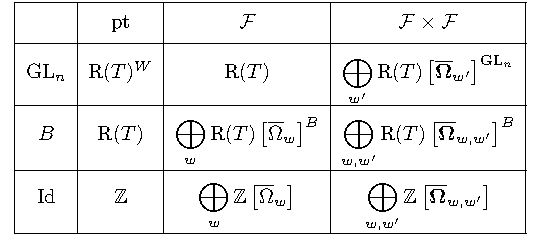
\includegraphics[width=8cm]{figures/table/table_module_initial.pdf}
      \caption[Module structure of $K$-theory: initial case]{Initial case}
      \label{table:module_initial}        
\end{table}
\begin{table}[ht]
  \vspace{0cm}
    \centering  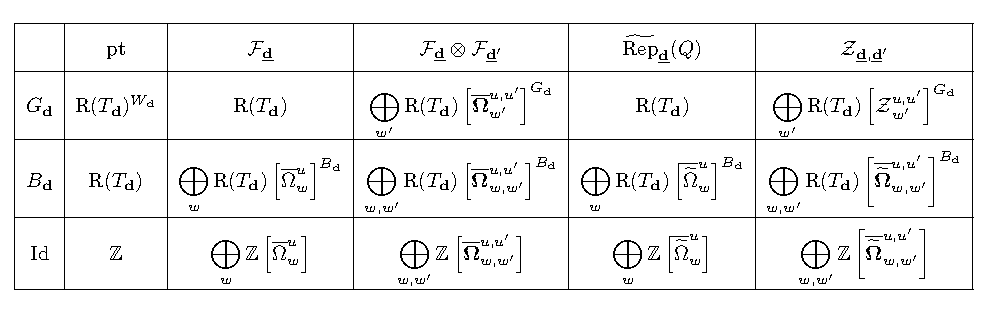
\includegraphics[width=15cm]{figures/table/table_module_relative.pdf}
      \caption[Module structure of $K$-theory: relative case]{Relative case}
      \label{table:module_relative}        
\end{table}
\begin{table}[ht]
  \vspace{0cm}
    \centering  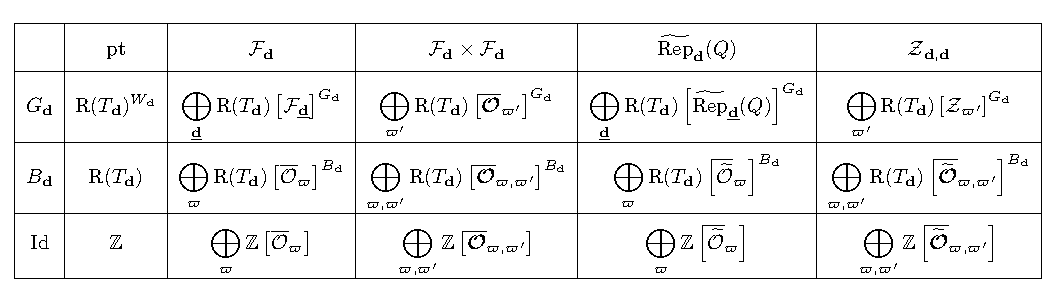
\includegraphics[width=15cm]{figures/table/table_module_absolute.pdf}
      \caption[Module structure of $K$-theory: absolute case]{Absolute case}
      \label{table:module_absolute}        
\end{table}
\clearpage
First, we work over Setting \ref{set:initial_case}.
\begin{eg}\label{eg:module-1-F}
The complete flag variety $\mathcal{F}$ has a stratification $\mathcal{F} = \sqcup_{w} \Omcell_{w}$. By extending the Bruhat order on $W$ to a total order $\preccurlyeq$, we get a cellular decomposition of $\mathcal{F}$:
% https://q.uiver.app/?q=WzAsMyxbMSwwLCJcXHN1YnNldGVxIFxcYmlnc3FjdXBfe3ggXFxwcmVjY3VybHllcSB3fVxcT21jZWxsX3t4fSBcXHN1YnNldGVxICJdLFswLDAsIjAgXFxzdWJzZXRlcSBcXE9tY2VsbF97XFxJZH0gXFxzdWJzZXRlcSJdLFsyLDAsIlxcc3Vic2V0ZXEgXFxiaWdzcWN1cF97eCB9XFxPbWNlbGxfe3h9ID1cXG1hdGhjYWx7Rn0iXSxbMSwwLCJcXGNkb3RzIiwzLHsic3R5bGUiOnsiYm9keSI6eyJuYW1lIjoibm9uZSJ9LCJoZWFkIjp7Im5hbWUiOiJub25lIn19fV0sWzAsMiwiXFxjZG90cyIsMyx7InN0eWxlIjp7ImJvZHkiOnsibmFtZSI6Im5vbmUifSwiaGVhZCI6eyJuYW1lIjoibm9uZSJ9fX1dXQ==
\[\begin{tikzcd}
	{0 \subseteq \Omcell_{\Id} \subseteq} & {\subseteq \bigsqcup_{x \preccurlyeq w}\Omcell_{x} \subseteq } & {\subseteq \bigsqcup_{x }\Omcell_{x} =\mathcal{F}}
	\arrow["\cdots"{marking}, draw=none, from=1-1, to=1-2]
	\arrow["\cdots"{marking}, draw=none, from=1-2, to=1-3]
\end{tikzcd}\]
By Theorem \ref{thm:cellular_fibration},
$$K^B(\mathcal{F}) \cong \bigoplus_{w} \Rpt(B) \left[ \overline{\Omcell}_{w} \right]^B \qquad K(\mathcal{F}) \cong \bigoplus_{w} \mathbb{Z} \left[ \overline{\Omcell}_{w} \right].$$
In particular,
\begin{equation*}
\begin{aligned}
  K^{\GL_n}(\mathcal{F} \times \mathcal{F}) \cong K^B(\mathcal{F})\cong\;& \bigoplus_{w} \Rpt(B) \cdot\Ind_B^{\GL_n} \left(\left[ \overline{\Omcell}_{w} \right]^B\right) \\ 
  \cong\;& \bigoplus_{w'} \Rpt(B)  \left[ \overline{\OOmcell}_{w'} \right]^{\GL_n}
\end{aligned}
\end{equation*}
\end{eg}


\begin{eg}\label{eg:module-2-FF}
$\mathcal{F} \times \mathcal{F}$ has many stratifications. Consider the stratification $\mathcal{F}\times \mathcal{F}= \sqcup_{w, w'\in W} \OOmcell_{w,w'}$. By extending the Bruhat order on $W \times W$ (i.e., $(x,x') \leqslant (w,w')$ if and only if $x \leqslant w$ and $x' \leqslant w'$) to a total order $\preccurlyeq$, we get a cellular decomposition of $\mathcal{F} \times \mathcal{F}$:
% https://q.uiver.app/?q=WzAsMyxbMSwwLCJcXHN1YnNldGVxIFxcYmlnc3FjdXBfeyh4LHgnKSBcXHByZWNjdXJseWVxICh3LHcnKX1cXE9PbWNlbGxfe3gseCd9IFxcc3Vic2V0ZXEgIl0sWzAsMCwiMCBcXHN1YnNldGVxIFxcT09tY2VsbF97XFxJZCxcXElkfSBcXHN1YnNldGVxIl0sWzIsMCwiXFxzdWJzZXRlcSBcXGJpZ3NxY3VwX3t4LHgnfVxcT09tY2VsbF97eCx4J30gPVxcbWF0aGNhbHtGfSBcXHRpbWVzIFxcbWF0aGNhbHtGfSJdLFsxLDAsIlxcY2RvdHMiLDMseyJzdHlsZSI6eyJib2R5Ijp7Im5hbWUiOiJub25lIn0sImhlYWQiOnsibmFtZSI6Im5vbmUifX19XSxbMCwyLCJcXGNkb3RzIiwzLHsic3R5bGUiOnsiYm9keSI6eyJuYW1lIjoibm9uZSJ9LCJoZWFkIjp7Im5hbWUiOiJub25lIn19fV1d
\[\begin{tikzcd}
	{0 \subseteq \OOmcell_{\Id,\Id} \subseteq} & {\subseteq \bigsqcup_{(x,x') \preccurlyeq (w,w')}\OOmcell_{x,x'} \subseteq } & {\subseteq \bigsqcup_{x,x'}\OOmcell_{x,x'} =\mathcal{F} \times \mathcal{F}}
	\arrow["\cdots"{marking}, draw=none, from=1-1, to=1-2]
	\arrow["\cdots"{marking}, draw=none, from=1-2, to=1-3]
\end{tikzcd}\]
By Theorem \ref{thm:cellular_fibration},
$$K^B(\mathcal{F} \times \mathcal{F}) \cong \bigoplus_{w,w'} \Rpt(B) \left[ \overline{\OOmcell}_{w,w'} \right]^B \qquad K(\mathcal{F} \times \mathcal{F}) \cong \bigoplus_{w,w'} \mathbb{Z} \left[ \overline{\OOmcell}_{w,w'} \right].$$

\end{eg}

\begin{eg}\label{eg:K-theory-by-induction}
For computing $K^{\GL_n}(\mathcal{F} \times \mathcal{F})$, consider the ($GL_n$-equivariant) stratification $\mathcal{F} \times \mathcal{F}= \sqcup_{w'} \OOmcell_{w'}$. Again, we get a cellular decomposition of $\pi_2: \mathcal{F} \times \mathcal{F} \longrightarrow \mathcal{F}$:
% https://q.uiver.app/?q=WzAsMyxbMSwwLCJcXHN1YnNldGVxIFxcYmlnc3FjdXBfe3gnIFxccHJlY2N1cmx5ZXEgdyd9XFxPT21jZWxsX3t4J30gXFxzdWJzZXRlcSAiXSxbMCwwLCIwIFxcc3Vic2V0ZXEgXFxPT21jZWxsX3tcXElkfSBcXHN1YnNldGVxIl0sWzIsMCwiXFxzdWJzZXRlcSBcXGJpZ3NxY3VwX3t4J31cXE9PbWNlbGxfe3gnfSA9XFxtYXRoY2Fse0Z9IFxcdGltZXMgXFxtYXRoY2Fse0Z9Il0sWzEsMCwiXFxjZG90cyIsMyx7InN0eWxlIjp7ImJvZHkiOnsibmFtZSI6Im5vbmUifSwiaGVhZCI6eyJuYW1lIjoibm9uZSJ9fX1dLFswLDIsIlxcY2RvdHMiLDMseyJzdHlsZSI6eyJib2R5Ijp7Im5hbWUiOiJub25lIn0sImhlYWQiOnsibmFtZSI6Im5vbmUifX19XV0=
\[\begin{tikzcd}
	{0 \subseteq \OOmcell_{\Id} \subseteq} & {\subseteq \bigsqcup_{x' \preccurlyeq w'}\OOmcell_{x'} \subseteq } & {\subseteq \bigsqcup_{x'}\OOmcell_{x'} =\mathcal{F} \times \mathcal{F}}
	\arrow["\cdots"{marking}, draw=none, from=1-1, to=1-2]
	\arrow["\cdots"{marking}, draw=none, from=1-2, to=1-3]
\end{tikzcd}\]
By Theorem \ref{thm:cellular_fibration} and Example \ref{eg:balanced_product_FF}, we get
\begin{equation*}
\begin{aligned}
  K^{\GL_n}(\mathcal{F} \times \mathcal{F})\cong\;& \bigoplus_{w'} K^{\GL_n}(\OOmcell_{w'})  \\ 
  \cong\;& \bigoplus_{w'} K^B(\Omcell_{w'})  \\ 
  \cong\;& \bigoplus_{w'} \Rpt(B) \left[ \overline{\OOmcell}_{w'} \right]^{\GL_n} \\ 
\end{aligned}
\end{equation*}
\end{eg}
The general case can be solved by the same method.
\begin{eg}
By repeating Example \ref{eg:K-initial-1} to \ref{eg:K-initial-4}, we get
$$\Rpt(N_{\dimvec{d}}) \cong \Rpt(\Id) \cong \mathbb{Z} \qquad \Rpt(B_{\dimvec{d}}) \cong \Rpt(T_{\dimvec{d}}) \cong \mathbb{Z}\!\left[ e_1^{\pm 1},\ldots,e_{\abdimvec{d}}^{\pm 1} \right]$$
$$ \Rpt(G_{\dimvec{d}}) \cong \Rpt(T_{\dimvec{d}})^{\Wd} \cong \mathbb{Z}\!\left[ e_1^{\pm 1},\ldots,e_{\abdimvec{d}}^{\pm 1} \right]^{\Wd}$$
The induction formula tells us 
$$K^{G_{\dimvec{d}}} (\mathcal{F}_{\ftdimvec{d}}) \cong K^{B_{\dimvec{d}}} (\pt) =\Rpt (B_{\dimvec{d}}) \cong \mathbb{Z}\!\left[ e_1^{\pm 1},\ldots,e_{\abdimvec{d}}^{\pm 1} \right].$$
By repeating Example \ref{eg:module-1-F} to \ref{eg:module-2-FF}, we get

\begin{equation*}
\begin{aligned}
&K^{B_{\dimvec{d}}}(\mathcal{F}_{\ftdimvec{d}}) \cong \bigoplus_{w} \Rpt(B_{\dimvec{d}}) \left[ \overline{\Omcell}_{w}^{u} \right]^{B_{\dimvec{d}}} \qquad &&K(\mathcal{F}_{\ftdimvec{d}}) \cong \bigoplus_{w} \mathbb{Z} \left[ \overline{\Omcell}_{w}^{u} \right]\\
&K^{G_{\dimvec{d}}}(\mathcal{F}_{\ftdimvec{d}} \times \mathcal{F}_{\ftdimvec{d}'}) \cong \bigoplus_{w'} \Rpt(B_{\dimvec{d}}) \left[ \overline{\OOmcell}_{w'}^{u,u'} \right]^{G_{\dimvec{d}}}\\
&K^{B_{\dimvec{d}}}(\mathcal{F}_{\ftdimvec{d}} \times \mathcal{F}_{\ftdimvec{d}'}) \cong \bigoplus_{w,w'} \Rpt(B_{\dimvec{d}}) \left[ \overline{\OOmcell}_{w,w'}^{u,u'} \right]^{B_{\dimvec{d}}} \qquad &&K(\mathcal{F}_{\ftdimvec{d}} \times \mathcal{F}_{\ftdimvec{d}'}) \cong \bigoplus_{w,w'} \mathbb{Z} \left[ \overline{\OOmcell}_{w,w'}^{u,u'} \right]\\
\end{aligned}
\end{equation*}

Since 
$$\mathcal{F}_{\dimvec{d}}= \bigsqcup_{\ftdimvec{d}}\mathcal{F}_{\ftdimvec{d}}\qquad \mathcal{F}_{\dimvec{d}} \times \mathcal{F}_{\dimvec{d}} = \bigsqcup_{\ftdimvec{d},\ftdimvec{d}'}\mathcal{F}_{\ftdimvec{d}} \times \mathcal{F}_{\ftdimvec{d}'}$$
as topological spaces, we get $K$-theory of $\mathcal{F}_{\dimvec{d}}$ and $\mathcal{F}_{\dimvec{d}} \times \mathcal{F}_{\dimvec{d}}$ for free. (See Table \ref{table:module_absolute})
\end{eg}

The calculations of incidence spaces use the same method we introduced in Example \ref{eg:K-theory-by-induction}.

\begin{eg}
We compute $G_{\dimvec{d}}$-equivariant $K$-theory of the Steinberg variety in this example.
\begin{equation*}
\begin{aligned}
  K^{G_{\dimvec{d}}}(\St_{\ftdimvec{d},\ftdimvec{d}'})\cong\;& \bigoplus_{w'} K^{G_{\dimvec{d}}}(\preimage{\OOmcell}_{w'}^{u,u'})  \\ 
  \cong\;& \bigoplus_{w'} K^{G_{\dimvec{d}}}(\OOmcell_{w'}^{u,u'})  \\ 
  \cong\;& \bigoplus_{w'} K^{B_{\dimvec{d}}}(\Omcell_{w'}^{u,u'})  \\ 
  \cong\;& \bigoplus_{w'} \Rpt(B_{\dimvec{d}}) \left[ \overline{\preimage{\OOmcell}}_{w'}^{u,u'} \right]^{G_{\dimvec{d}}} \\ 
\end{aligned}
\end{equation*}
\end{eg}

The equivariant cohomology theory can be computed in the same way, see \cite[Chapter 7]{przezdziecki2015geometric}.
